% !TeX spellcheck = en_GB
\documentclass{article}
\pdfpagewidth=8.5in
\pdfpageheight=11in

\usepackage{kr}
\usepackage{kr-MlLogicApi}

\pdfinfo{
/TemplateVersion (KR.2022.0)
}

%\title{Towards a Logic Programming library for Machine Learning: API design and prototyping}
\title{
    Logic Programming library for Machine Learning:
    \\
    API design and prototype
}

\author{%
    Giovanni Ciatto
    \and
    Matteo Castigliò
    \and
    Roberta Calegari
    \\
    \affiliations
    $^1$Departement of Computer Science and Engineering (DISI) %, Alma Mater Studiorum---Università di Bologna
    \\
    $^3$Alma Mater Research Institute for Human Centered AI (AlmaAI)
    \\
    $^{1,3}$Alma Mater Studiorum---Università di Bologna
    \\
    \emails\ttfamily
    $^{1,3}$\{giovanni.ciatto, roberta.calegari\}@unibo.it,
    $^{2}$matteo.castiglio@studio.unibo.it
}

\begin{document}

\maketitle

\begin{abstract}
%Deductive inference is amongst the most prominent features for making a system intelligent.
%%
%Logic programming enables the representation and automatic manipulation of reasoning, via sequences of implications.
%%
%While this approach supports the creation of inherently-comprehensible systems (for the human mind), it may result inadequate to tackle complex or large corpi of knowledge.
%%
%Conversely, modern artificial neural networks support the automatic provisioning of knowledge from experience, via machine learning.
%%
%The latter approach is highly scalable, as it does not require logic knowledge to be handcrafted by humans.
%%
%Unfortunately, however, it leads to poorly interpretable systems and it requires large amounts of data to be available.
%%
%The two approaches are thus complementary.

In this paper we address the problem of hybridising symbolic and sub-symbolic approaches in artificial intelligence, following the purpose of creating flexible and data-driven systems, which are simultaneously comprehensible and capable of automated learning.
%
In particular, in this paper we propose a logic API for supervised machine learning, enabling logic programmers to exploit neural networks -- among the others -- in their programs.
%
Accordingly, we discuss the design and architecture of a library reifying APIs for the Prolog language in the \twopkt{} logic ecosystem.
%
Finally, we discuss a number of snippets aimed at exemplifying the major benefits of our approach when designing hybrid systems.

\end{abstract}

%----------------------------------------------------------------------------------------
\section{Introduction}
\label{sec:introduction}
%---------------------------------------------------------------------------------------

Symbolic and sub-symbolic artificial intelligence (AI) are complementary under a number of perspectives \cite{ilkou2020symbolic,xaisurvey-ia14}.
%
%The same is true for their major techniques, namely logic programming (LP) and neural networks (NN).
%
For this reason, many recent contributions from the literature are discussing the possible frameworks for their integration and hybridisation \cite{BarredoArrieta2020,Goertzel2012,lpaas-bdcc2,xailp-woa2019}.
%
However, what is currently slowing down scientific progress in this context is not the lack of ideas concerning \emph{how} such integration and hybridisation may occur.
%
Conversely, the bottleneck is caused by the lack of suitable technologies enabling and easing the experimentation of integrated or hybrid systems.
%
Logic-based technologies are in fact technological islands, for which poor care is given to the construction of bridges with the rest of the AI land.

Accordingly, in this paper, we address the issue of supporting machine learning (ML) -- and, in particular, neural-networks (NN) based training and inference -- in logic programming (LP).
%
We do so by designing and prototyping a logic based API for machine learning.
%
Along this line, our contribution is twofold:
%
\begin{inlinelist}
    \item we let logic programmers exploit the benefits of sub-symbolic AI, and, in particular, neural networks; and
    \item we enable the practical experimentation of hybrid systems---involving both logic and neural processing of data.
\end{inlinelist}

Our logic-based API for ML consists of a set of logic predicates enabling the representation, training, testing, and exploitation of sub-symbolic predictors in LP---possibly, out of data expressed in logic form.
%
In other words, our API lets logic programmers use neural networks in their programs -- e.g. to train or exploit classifiers or regressors -- without requiring them to abandon the logic realm.
%
Of course, to make this possible, our API supports the whole gamma of low level tasks that are commonly involved in an ML workflow---including, but not limited to, data preprocessing, cross-validation, etc.

%RC: qui sotto metterei giusto una coppia di frasi che riassumono la tech usata, con i riferimenti
Technically, we prototype our API via a logic library -- namely, the \mllib{} -- targetting the \twopkt{} ecosystem \cite{2p-kt}, and the JVM platform.
%
%It consists of a number of primitives bridging the logic realm with some underlying machine-learning library, allowing Prolog to manipulate sub-symbolic facilities such as datasets, neurons, layers, or activation functions, and vice versa.
%
\deeplearningforj{} \cite{DL4J} is the underlying library we leverage upon in this paper.
%
However, our design is general enough to support other libraries and, possibly, different platforms---e.g. Tensorflow \cite{tensorflow2015-whitepaper} over Python.

Arguably, our work represents the first step towards a wider degree of interoperability among symbolic- and sub-symbolic AI.
%
In fact, one the long run, we aim to enable the design and construction of hybrid systems, fruitfully and dynamically combining the major advantages of both approaches to artificial intelligence by mixing inferential (via LP) and intuitive (via NN) reasoning capabilities.
%
Along this path, the proposed API is a key enabling factor, as it supports the creation of logic-based inferential engines which are capable of learning from data via state-of-the-art mechanisms.
%
Dually, by supporting the training of neural networks from logic data, our API can also be considered as a tool for endowing sub-symbolic predictors with prior, high-level knowledge.

%Accordingly, the reminder of this paper is organised as follows.
%%
%In \cref{sec:requirements}, we describe and analyse the supervised ML domain, with the purpose of identifying which functionalities our logic API for ML should support, and how exactly they are expected to work.
%%
%Then, in \cref{sec:project}, we delve into the design of the \mllib{} discussing and motivating conventions, syntactic choices, and architectural decisions.
%%
%In \cref{sec:tech}, we then discuss a number of technology- and platform-related aspects arising when prototyping the \mllib{}.
%%
%There, we motivate technological commitments such as \twopkt{} and \deeplearningforj{}.
%%
%\cref{sec:examples} is where we discuss a number of examples concerning the usage of the \mllib{}, and its potential applications.
%%
%Finally, \cref{sec:conclusions} concludes the paper, providing some insights about the future research directions stemming from this work.
%

%----------------------------------------------------------------------------------------
\section{Logic library for ML: goals}\label{sec:goals}
%----------------------------------------------------------------------------------------

To properly design a logic library for dealing with hybrid reasoning, some basic goals to achieve should be taken into account: namely,
%
\begin{inlinelist}
    \item enable hybrid reasoning,
    \item full support of declarative ML,
    \item enable the exploitation of symbolic data sources (in addition to the others),
    \item make it possible to select a model via resolution.
\end{inlinelist}
%
It is worth mentioning that, each one of these goals comes along with some of the benefits of hybridization, discussed in detail in \cite{xaisurvey-ia14}.
%
In the following details about these goals are discussed.

\paragraph{Hybrid reasoning}
%
Automatic reasoning may greatly benefit from sub-symbolic AI to overcome its inherent crispness.
%
Fuzzy data could then be suitably and coherently processed by a sub-symbolic predictor as part of a wider symbolic resolution process.
%
To make this possible, sub-symbolic predictors should be representable, trainable, and queryable as any other logic predicate, without requiring the semantics of logic resolution to be affected.
%
Consequently, logic programs should be endowed with ad-hoc predicates and syntactical categories, aimed at representing and manipulating sub-symbolic predictors and data.

\paragraph{Declarative ML} Declarative ML is a paradigm by which data scientists' code should only specify \emph{what} an ML workflow should do, by leaving the underlying platform in charge to understand \emph{how}.
%
This is partially supported by the current practice of data science which relies on high-level languages (e.g. Python) and libraries of elementary components to be composed (e.g. Scikit-Learn by \citeay{scikit-learn}).
%
However, the solutions proposed so far do not leverage inherently declarative frameworks like LP, but rather object-oriented languages---requiring imperative statements.
%
Hence, to support the declarative expression of an ML workflow in the LP framework, a new logic API is required.
%
%This would be useful both from a logic and ML perspective.
%%
%In fact, it would pave the way towards the exploitation of ML within the LP community, other than providing data scientists with a way to describe their ML workflows in a formal and runnable way.

\paragraph{Symbolic data sources}
%
Logic knowledge bases are a peculiar way of collecting knowledge.
%
Unlike datasets and DBMS, they represent information in symbolic form, via -- possibly \emph{intensional} -- logic formul\ae{}.
%
Hence, they can virtually represent any sort of datum -- be it atomic, compound or structured -- via a concise (yet very expressive) language, while possibly saving space.
%
Accordingly, when combining LP with ML, knowledge bases should be exploitable as data sources as well---other than ordinary CSV files or relational databases.

\paragraph{Model selection via resolution}
%
Logic resolution essentially consists of a search procedure aimed at finding solutions in a proof tree.
%
This could be applied to a common step of any ML workflow---namely \emph{model selection}.
%
There, data scientists must assess several predictor families, to select the one which is better suited for the learning task at hand.
%
Then, they must search for the best hyper-parameters for the selected family of predictors.
%
All such choices involve several sorts of predictors, with possibly different hyper-parameters, to be trained and compared---either in an orderly fashion or in parallel.
%
LP naturally captures the non-deterministic exploration of a space of possible choices.
%
Hence it is well suited to both declaratively represent and implement model selection.

%----------------------------------------------------------------------------------------
\section{ML: key aspects to be supported}
\label{sec:requirements}
%----------------------------------------------------------------------------------------

To support the aforementioned goals, logic APIs must cover the full gamma of aspects involved in any possible ML workflow, detailed and discussed in this section.

Briefly speaking, a ML workflow is the process of producing a suitable predictor for the available data and the learning task at hand, following the purpose of later exploiting that predictor to draw analyses or to drive decisions.
%%
%Hence, any ML workflow is commonly described as composed by two major phases, namely training -- where predictors are fit on data -- and inference---where predictors are exploited.
%%
%However, in practice, further phases are included, such as data provisioning and preprocessing, as well as model selection and assessment.
%%
%
Each ML workflow can be conceived as composed by six major phases -- elicited in \cref{ssec:ml-phases} --, each one involving a number of activities---elicited in \cref{ssec:modelling}.
%
Enumerating and defining all possible phases and activities is of paramount importance, as any API for ML should support them all.

\subsection{ML phases}
\label{ssec:ml-phases}

From a coarse-grained perspective, a machine learning workflow is composed by six major phases, detailed in the following.

\paragraph{Dataset loading}
%
%Provided that the data provisioning phase has resulted in a dataset -- roughly, a collection of homogenous data, often coming in the form of a single file, a folder or a database --,
The first step of any ML workflow consists of loading that dataset in memory for later processing.
%
To support such a step, ML frameworks come with ad-hoc functionalities aimed at loading the dataset by reading a file from the local file system, by fetching it from the Web, or by querying a DBMS.
%
These usually come in the form of either classes or functions, coherently w.r.t. the object-oriented nature of mainstream ML frameworks.
%
Accordingly, the logic API for ML should expose ad-hoc \emph{predicates} to serve the same purposes.
%
Furthermore, however, it should also support the loading of datasets out of logic theories of facts and rules.

\paragraph{Data pre-processing}
%
Raw datasets are often inadequate to favour predictors' training.
%
Hence, dataset pre-processing is commonly practised to increase the effectiveness of any subsequent training phase.
%
Pre-processing most common bulk operations are:
%
\begin{inlinelist}
    \item homogenize the variation ranges of the many features sampled by the dataset,
    \item detect irrelevant features and remove them,
    \item construct relevant features by combining the existing ones,
    \item encoding non-numeric features into numeric form, and
    \item\label{preprocessing:partitioning} horizontal (by row) or vertical (by column) partitioning of the dataset.
\end{inlinelist}
%
In particular, the purpose \ref{preprocessing:partitioning} is of paramount importance, as it supports the \emph{test set separation} as well as splitting input-related columns from output-related ones---fundamental operation to enable validation and testing and to support training respectively.

\paragraph{Predictor selection and definition}
%
Many sorts of predictors could be used in principle to perform supervised learning---e.g. neural networks, decision trees, support vector machines, etc.
%
A preliminary phase to select the best predictor is a common phase in virtually any ML workflow.
%
Once a particular sort of predictor has been chosen, a way to specify the shape the to-be-trained predictor should have is required.
%
Of course, such specification should take into account the schema of the input data, as well as the schema of the expected outcomes to be produced by the predictor.
%
Finally, \emph{hyper-parameters} of the selected algorithm need to be tuned.
%
%Consider the case of neural networks as an example.
%%
%Decision points in this case concern the choice of
%%
%\begin{inlinelist}
%    \item which and how many hidden layers (of neurons) to adopt,
%    \item how to interconnect them, and
%    \item which activation functions to adopt for the neurons therein contained.
%\end{inlinelist}

Accordingly, the logic API for ML should support the specification of as many sorts of predictors as possible, as well as their parametrisation.
%
Once again, predicates should be defined to serve this purpose.
%
In particular, at least one ad-hoc predicate should be defined for each sort of predictor to be supported, carrying as many arguments as the possible hyper-parameters that could be specified for that sort of predictor.
%
In case hyper-parameters cannot be conveniently represented as raw logic types (numbers or strings), ad-hoc predicates should be provided as well for constructing structured hyper-parameters values.

%In the particular case of neural networks, ad-hoc predicates should be provided to construct layers, and activation functions, and to combine them to create arbitrarily complex network architectures.

\paragraph{Training}
%
Predictors' training plays a pivotal role in ML workflows.
%
This is the phase where predictors are fit on the available data or, in other words, automated learning actually occurs.
%
Generally speaking, training can be modelled in LP as a single predicate, mapping untrained predictors into trained ones, possibly via a number of learning parameters (e.g. learning rate or momentum for NN, or maximum depth for DT), or stopping criteria (e.g. max epochs for NN, or max depth for DT), other than, of course, the data to be used for training.
%
Once again, several ad-hoc predicates should be defined to support structured parameters or stopping criteria in the logic API for ML.
%
Furthermore, regardless of its shape, the training predicate should accept some arguments aimed at specifying whether the columns of the training set should be considered as inputs or outputs.

\paragraph{Inference}
%
Inference is commonly the last phase of any ML workflow.
%
Here, trained predictors are used to draw predictions on new data---i.e. different data w.r.t. the training set.
%
%In particular, given a raw datum having the same schema of the input data used for training -- there including any prior pre-processing phase --, the trained predictor can be exploited to compute the corresponding prediction---even if (and especially because) the raw datum has never been observed before by that predictor.
%
In most common cases, predictions attempt to solve classification or regression problems.
%
In any case, yet another general predicate should be added to our logic API for ML to support drawing predictions out of a trained predictor and a set of raw data (or a single datum).
%
Ad-hoc predicates may be provided as well to explicitly model higher-level tasks, such as classification and regression.
%
Finally, it should be possible to store, retrieve, and re-apply any pre-processing procedure possibly defined before training, to the raw data for which predictions should be drawn---in order to make it acceptable for the predictor as an input.

\paragraph{Validation}
%
Validation is the \emph{penultimate} step of any ML workflow: it succeeds training and precedes exploitation.
%
It is here discussed as last because it technically relies on the capability of drawing predictions via trained predictors---which is treated in the paragraph above.

Generally speaking, validation attempts to measure the predictive performance of a trained predictor, with the purpose of assessing if and to what extent it will generalise to new, unseen data.
%
To this end, the predictor is tested against the test set---that is, a collection of unseen data, for each expected predictions exist.
%
The discrepancy (or similarity) among the actual and expected predictions is then measured via ad-hoc scoring functions (a.k.a. measures), resulting in a performance assessment for the trained predictor.
%
Many measures may be used to assess classifiers (e.g. accuracy, F1-score, etc.) and as many to assess regressors (e.g. MAE, MSE, R$^2$, etc.).
%
Hence, to support validation, the logic API for ML should provide predicates to compute each possible measure.

%----------------------------------------------------------------------------------------
\subsection{ML activities, per phase}
\label{ssec:modelling}
%----------------------------------------------------------------------------------------

Here we elicit the many activities involved in each phase of any ML workflow, and we describe them from a computational perspective---i.e. in terms of the sorts entities (a.k.a. data types) they accept as input or produce as output (manipulate, for short).

\paragraph{Entities}

We start our discussion by identifying the five major sorts of entities each activity may manipulate.
%
\begin{itemize}
	\item \emph{Value:} a scalar, vectorial, matrix, or tensorial datum from a given domain (e.g. integer or real numbers, or vectors of integer or real numbers, as well as a string, a table, a time series, etc.).
	%
	\item \emph{Schema:} a concise and formal description of a domain (i.e. a set of values).
	%
	For scalar values, schemas are essentially data types (e.g. integers, reals, strings, etc.), while for non-scalar data they carry information about the name, index, and type of each single scalar component.
	%
	\item \emph{Dataset:} a collection of values matching a particular schema (supposed to be known).
	%
	\item \emph{Transformation:} any operation aimed at transforming an entity dataset into another other---commonly, a dataset into either another dataset (e.g. normalization, standardization, etc.) or a value (e.g. max, min, average, etc.)
	%
	From an algebraic perspective, it is a function.
	%
	From a computational perspective, it is an algorithm.
	%
	\item \emph{Predictor:} a stateful computational entity capable of
	%
	\begin{inlinelist}
		\item drawing predictions (i.e. outputting values) out of (possibly unseen) input values, according to its internal state
		\item updating its internal state according to a dataset (to improve future predictions)
	\end{inlinelist}
\end{itemize}
%
Any logic-based API for ML should support the representation, combination, and manipulation of entities of these kinds.

\paragraph{Activities}

Each phase of the ML workflow is then characterised by a specific set of activities possibly manipulating entities of any of these sorts.
%
A logic-based API for ML should support them as well.
%
Accordingly, in the remainder of this section, we describe such activities along with the entities they operate upon.
%
In doing so, we partition activities w.r.t. the ML phase they are most commonly exploited into.

\subparagraph{Dataset loading}
%
The main activities to support the loading of a dataset into a solver's memory, and its preparation for subsequent processing are
%
\begin{itemize}
    \item \emph{Dataset loading:} operation of loading a dataset from either a value -- representing either a local or remote file --, or from a Prolog theory
    \item \emph{Schema declaration:}  operation of constructing a representation for a given schema
    \item \emph{Target features declaration:} operation of tagging a portion of the features of some schema as either inputs or outputs (a.k.a. targets)
    \item \emph{Dataset splitting:} operation of horizontally partitioning a dataset into two or more smaller datasets.
\end{itemize}

\subparagraph{Dataset pre-processing}
%
Here, they may be willing to define transformations or cascades of transformations (pipelines, henceforth) to be eventually applied on datasets:
%
\begin{itemize}
    \item \emph{Transformation declaration:} operation of declaratively encoding a transformation operation to be applied to all data in a dataset
    %Such kinds of transformations can be modelled as functions accepting a dataset as input and producing a dataset as output
    \item \emph{Pipeline composition:} operation of declaratively constructing a composite transformation as a cascade of simpler transformations
    \item \emph{Transformation application:} operation of actually constructing a new dataset from a prior dataset and a transformation
\end{itemize}

\subparagraph{Predictor selection and definition}
%
The next phase involves the \emph{definition} of one or more predictors via a unique meta-activity, namely:
%
\begin{itemize}
    \item \emph{Predictor declaration:} operation of constructing a representation for a particular predictor, which implies choosing the predictor family and specifying actual values for its hyper parameters
\end{itemize}
%%
%Of course, as many families of predictors exist, and each one is characterised by its own set of formal hyper-parameters, many variant if this operation may eventually be defined in practice.

\subparagraph{Training}
%
Eventually, declared predictors may enter the \emph{training} phase, meaning that their learning from data should be triggered.
%
This can be achieved via yet another activity, namely:
%%
\begin{itemize}
    \item \emph{Predictor fitting w.r.t. a training set of data:} operation of fitting a predictors' internal parameter on some provided training data
\end{itemize}
%%
%Again, given the variety of predictors available, this operation may come with several predictor specific variants accepting different learning parameters.

\subparagraph{Inference}
%
Once in their \emph{inference} phase, trained predictors may eventually be exploited to draw predictions.
%%
The corresponding activity is:
%%
\begin{itemize}
    \item \emph{Predictor querying:} operation where (possibly unseen) values are provided to some trained predictor as a query, and the resulting values are interpreted as predictions
\end{itemize}

\subparagraph{Validation}
%
Finally, in the \emph{validation} phase, trained predictors should be assessed by measuring their performance w.r.t. some test data
%
This is yet another meta-activity, with several possible variants depending on the particular measure being exploited:
%
\begin{itemize}
    \item \emph{Predictor scoring:} operation of computing a scoring value out of a trained predictor, a test dataset, and a scoring function
\end{itemize}

%----------------------------------------------------------------------------------------
\section{\mllib{} Overview and Architecture}
%----------------------------------------------------------------------------------------

\begin{figure}
    \centering
    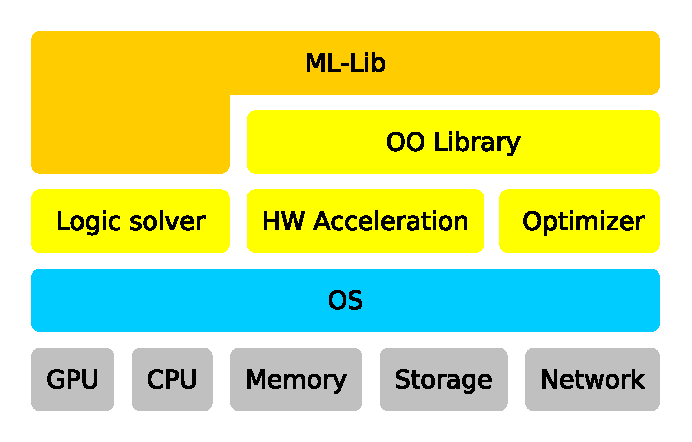
\includegraphics[width=\linewidth]{figures/layers.pdf}
    \caption{Layered view of the proposed \mllib{}. An OO library is assumed behind the scenes, providing high-level abstraction to optimize ML predictors, possibly via HW acceleration.}
    \label{fig:layers}
\end{figure}

This section discusses the design of \mllib, the logic programming library reifying the logic API for ML reifying the meta-model discussed above.
%
The overall architecture is depicted in \cref{fig:layers}.
%
The \mllib{} assumes a goal-oriented logic solver being in place, where ordinary logic programs can be executed.
%
Thanks to the \mllib{}, these logic programs may also exploit a number of predicates for training and using ML predictors---other than any other entity involved in the process.

In the backend, the library assumes an underlying object-oriented (OO) library providing high-level ML abstractions, such as datasets, predictors, and so on.
%
Examples of these libraries may be for instance Keras \cite{chollet2015keras} or \deeplearningforj{} \cite{DL4J}.
%
The OO library may in turn be backed by an optimizer taking care of making training and data management effective on the available hardware---and possibly exploiting hardware acceleration.
%
In practice, software such as Theano, Caffe, or Tensorflow may serve this purpose.
%
Actual technological choices may finally depend on the particular runtime platforms being targeted.
%
For instance, targeting the JVM may imply \deeplearningforj{} to be exploited, while targetting Python may exploit both Keras and Tensorflow.
%
However, while technological choices are contingent and subject to change, the overall architecture is meant to support the implementation of the \mllib{} as a façade towards the underlying OO library, regardless of what it is.

At the functional level, the design of the \mllib{} is provided in terms of logic predicates acting on the above defined entities.
%
Details about the predicates are provided in the supplementary material.
%
\Cref{fig:design-overview} provides an overview of these predicates, grouped by entities.

\begin{figure*}
    \centering
    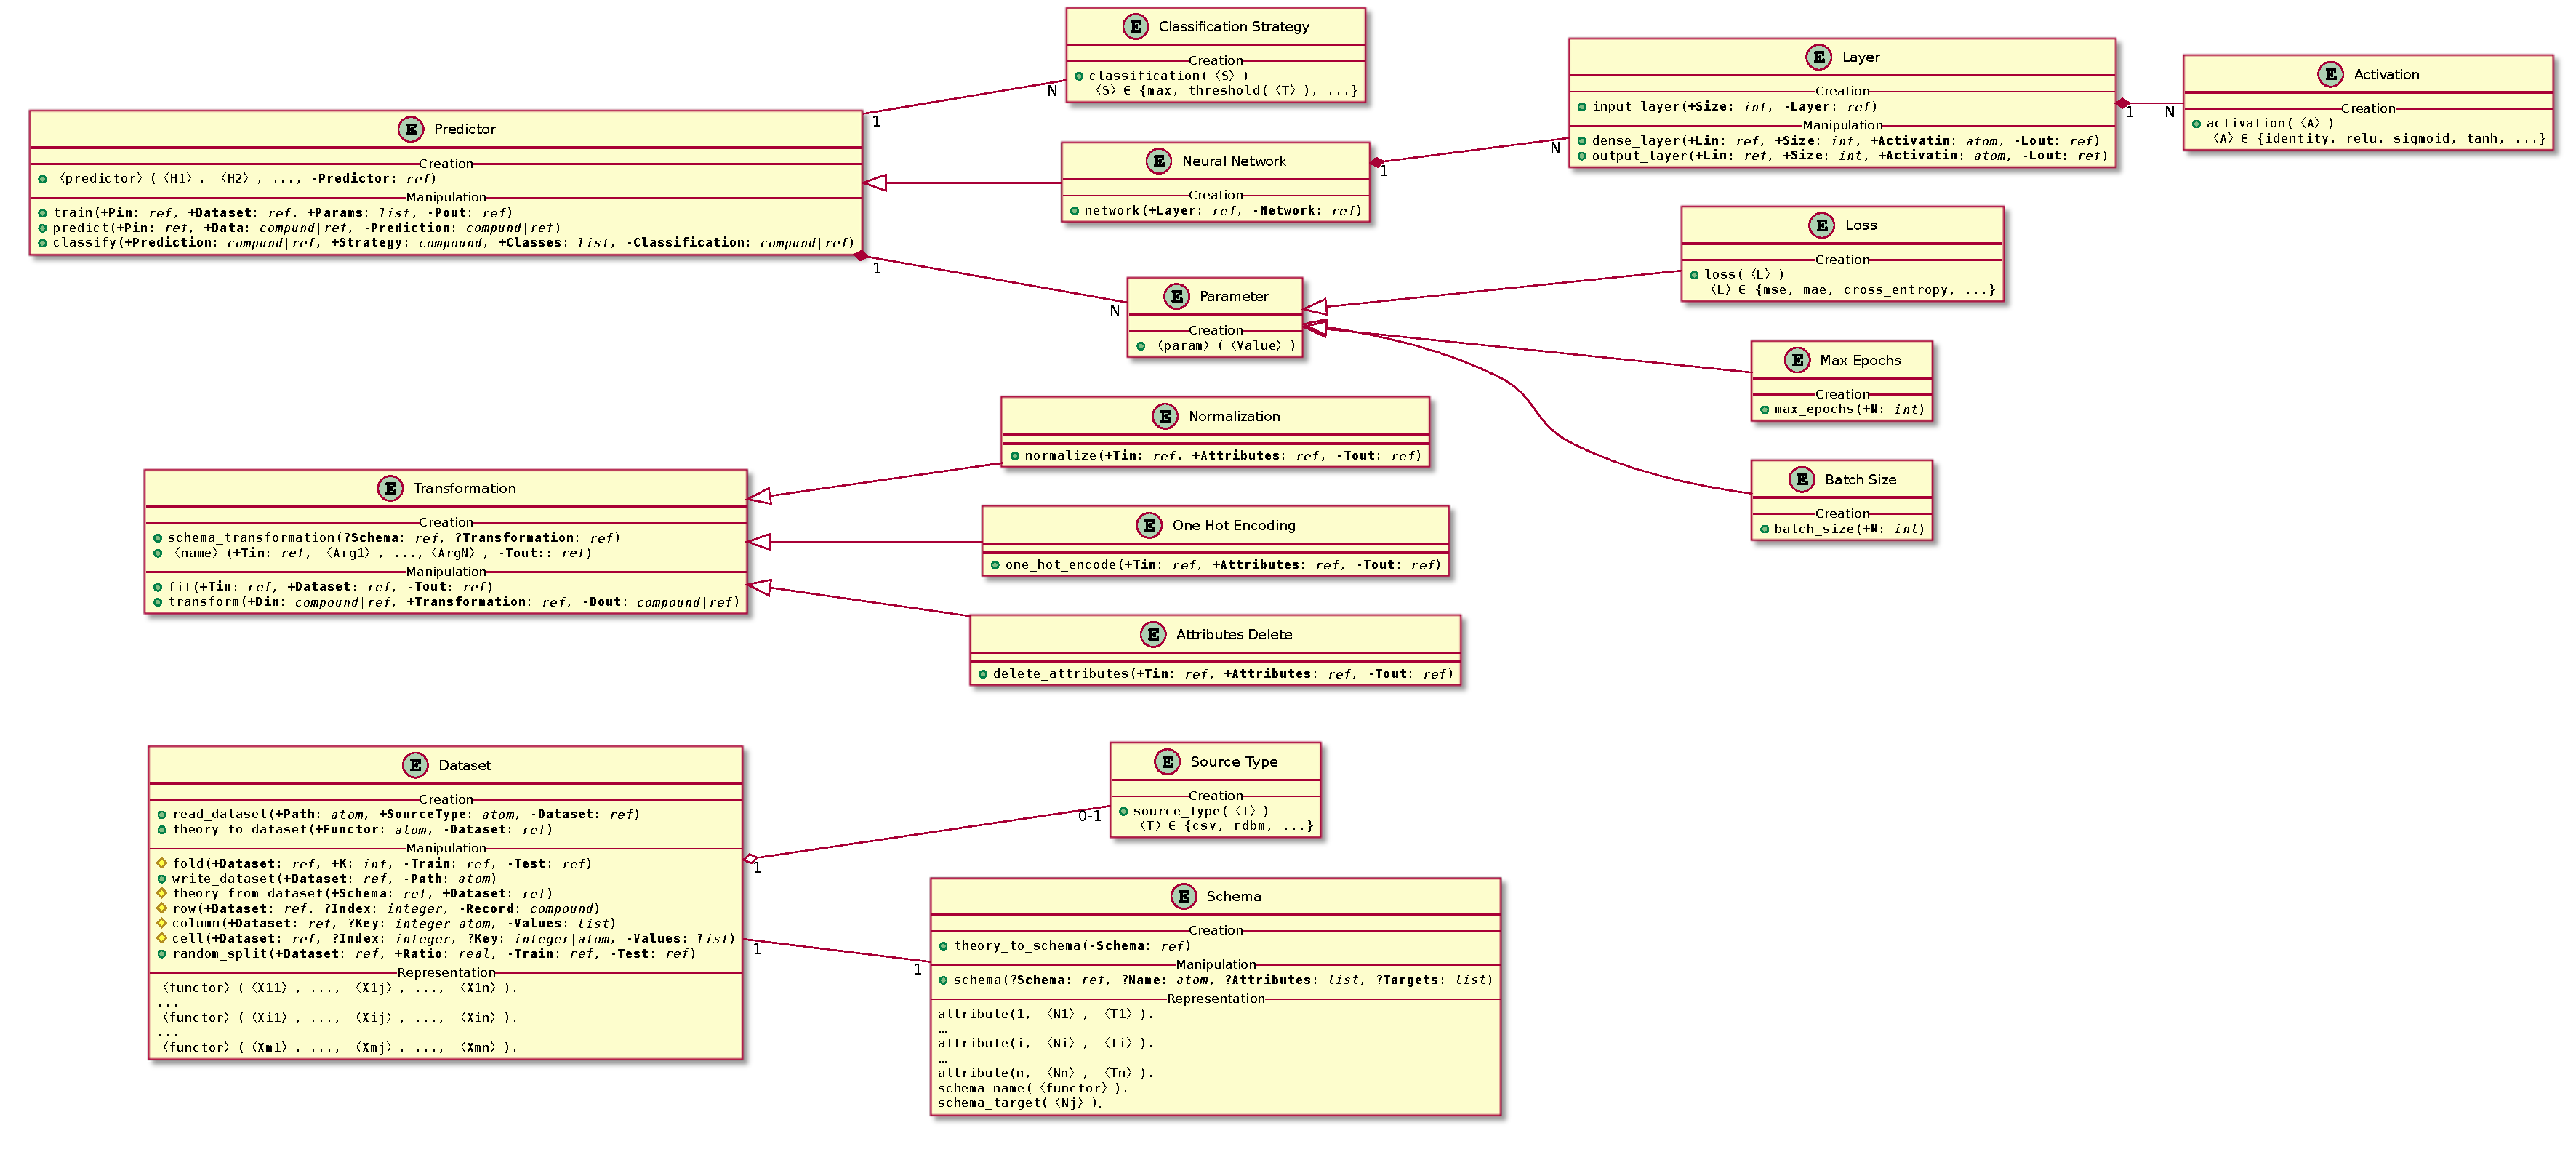
\includegraphics[width=\linewidth]{figures/entities.pdf}
    \caption{Overview of our \mllib{} design. The chart represents the many entities logic programmers may exploit via our \mllib{}, and the many predicates supporting their creation, manipulation, or representation. Predicates are depicted with either a yellow diamond in case they are non-deterministic (a.k.a. backtrackable), or a green circle otherwise.}
    \label{fig:design-overview}
\end{figure*}

%----------------------------------------------------------------------------------------
\section{\mllib{} Examples}
\label{sec:examples}
%----------------------------------------------------------------------------------------

Here we discuss the usage of the \mllib{} to serve the purposes described in \cref{sec:goals}.

From an LP perspective, our examples assume the existence of a logic solver/language exploiting some implementation of the \mllib{}.
%
For the sake of simplicity, we assume a Prolog solver is employed.
%
Examples consist of Prolog scripts, possibly involving standard Prolog predicates.

From an ML perspective, our examples assume a very simple scenario where a neural-network classifier is trained on the well known Iris dataset \cite{iris-dataset}.
%
The resulting NN is then exploited to write a simple hybrid predicate aimed at classifying unseen Iris instances.

\paragraph{Declarative ML}
%
Declarativeness is a key benefit of our symbolic approach to ML.
%
The \mllib{} supports declarative ML in several ways, as exemplified by listings \ref{lst:dataset-loading}, \ref{lst:pre-processing-pipeline}, \ref{lst:neural-network-declare}, and \ref{lst:training}.

%\begin{figure}
    \prologimport[
%        captionpos=b,
        label={lst:dataset-loading},
        caption={Dataset loading from file}
    ]{listings/dataset-loading.pl}
    %
    \prologimport[
        label={lst:pre-processing-pipeline},
        caption={Pre-processing pipeline}
    ]{listings/pre-processing-pipeline.pl}
    %
    \prologimport[
        label={lst:neural-network-declare},
        caption={Neural network structure declaration}
    ]{listings/neural-network-declare.pl}
%\end{figure}

In particular, \cref{lst:dataset-loading} shows how the schema and data entries of the Iris dataset can be treated in logic.
%
Notably, the Iris data set contains 150 rows describing as many individuals of the Iris flower.
%
For each exemplary, 4 continuous input attributes -- \emph{petal} and \emph{sepal width} and \emph{length} -- are recorded, other than a categorical target attribute---denoting the actual Iris \emph{species}.
%
There are three particular species of Iris in this data set -- namely, Setosa, Virginica, and Versicolor --, and the 150 examples are evenly distributed among them---i.e., there are 50 instances for each class.
%
The Prolog script describes the Iris dataset's schema in clausal form, as discussed in \cref{ssec:schemas}.
%
It also declares two predicates -- namely, \pl{iris\_schema/1} and \pl{iris\_dataset/1} -- aimed at letting the logic programmer retrieve either the schema or its dataset in object form.
%
More precisely, \pl{iris\_schema/1} attempts to read the schema from the local theory, while \pl{iris\_dataset/1} attempts the load the dataset from a CSV file.
%
\Cref{lst:logic-dataset-loading} (presented later in this section) reports a similar scenario where the dataset as well is loaded from the local theory.

\Cref{lst:pre-processing-pipeline} exemplifies the declaration of a pre-processing pipeline aimed at normalising the input attributes of any \pl{Dataset} having the same \pl{Schema} of Iris, other than one-hot encoding its output attributes.
%
The resulting \pl{Pipeline} is then fitted against the provided \pl{Dataset}, and bound to the corresponding output argument.

In turn, \cref{lst:neural-network-declare} presents a general purpose predicate aimed at defining multi-layered perceptron predictors with an arbitrary amount of hidden layers.
%
This is made possible by the \pl{multi\_layer\_perceptron/4} predicate, which requires the caller to provide the number of neurons to be instantiated for
%
\begin{inlinelist}
    \item the input layer (\pl{Nin}),
    \item the output layer (\pl{Nout}), and
    \item for each hidden layer (\pl{Nhidden}).
\end{inlinelist}
%
Notably, \pl{Nhidden} should consist of a list in integers, denoting the number of neurons for each hidden layer -- from the outermost to the innermost --, while the total amount of integers corresponds to the number of hidden layers.
%
The resulting neural network predictor is then bound to the \pl{NN} output argument.
%
So, for instance, a NN having 4 input neurons, 2 hidden layers with 5 and 7 neurons respectively, and 3 output neurons can be declared as follows:
%
\begin{lp}
    multi\_layer\_perceptron(4,[5, 7],3,NN)
\end{lp}

Finally, \cref{lst:training} declares an end-to-end ML workflow aimed at selecting and training the best NN architecture to tackle Iris classification.
%
It is worth noting that the declarative nature of the script can be regarded as a formal -- yet human-readable -- specification of a classifier training workflow.

\paragraph{Symbolic data sources}

As highlighted above it may be useful to perform ML upon data expressed in logic form.
%
This requires logic theories to act as symbolic data sources.
%
\mllib{} supports such scenario, as exemplified in \cref{lst:logic-dataset-loading}.
%
The script is assumed to replace \cref{lst:logic-dataset-loading} in those situations where the Iris dataset is logically described in the clausal form.
%
Here, the \pl{iris\_dataset/1} attempts to load the data from the local theory instead of a file.

\prologimport[
%    float,
    label={lst:logic-dataset-loading},
    caption={Dataset loading from the local theory}
]{listings/logic-dataset-loading.pl}

\paragraph{Model selection via resolution}
\label{par:model-selection}

The automatic exploration of a search space subtended by logic resolution could be exploited to perform model selection.
%
Indeed, model selection essentially consists of an exploration of the hyper and learning parameters space, looking for the best possible values---i.e. those hyper and learning parameters assignments corresponding to well-performing predictors on the available training set.

Accordingly, the \mllib{} supports expressing and performing model selection in logic (\cref{lst:training}).
%
%\medskip
\prologimport[
%    float,
%    captionpos=b,
    linewidth=1.07\linewidth,
    label={lst:training},
    caption={[Declarative description of a ML workflow]Declarative description of a ML workflow aimed at selecting the best hyper and learning parameters for a NN classifier. Ancillary predicates invoked in this snippet are reported in the supplementary material.}
]{listings/training.pl}
\bigskip
%
There hyper, learning, and workflow parameters are expressed as logic facts, and the \pl{params/2} predicate is defined to enumerate all possible combinations of theirs---e.g. via Prolog's backtracking mechanism.
%
The \pl{model\_selection/5} predicate is in charge of stepping through all such parameters with the purpose of selecting, and training all corresponding NN predictors which attain a sufficiently high predictive performance---denoted by the \pl{target\_performance/1} fact.
%
For each trained predictor, the predicate outputs not only a reference to the \pl{Predictor} itself, but also its \pl{Performance}, and the affine \pl{Transformation} to be applied to each datum for which predictions should be drawn using that predictor.
%
The predicate \pl{model\_selection/5} works by
%
\begin{enumerate}
    \item splitting the provided \pl{Dataset} into a \pl{TrainingSet} and a \pl{TestSet}, according to a split ratio (\pl{R}) declared by the \pl{test\_percentage/1} fact
    \item declaring and fitting a pre-processing \pl{Transformation} aimed at normalising the \pl{TrainingSet}'s input attributes, and one-hot encoding its output attributes
    \item applying such \pl{Transformation} to the \pl{TrainingSet}, hence producing a \pl{ProcessedTrainingSet}
    \item stepping through all possible hyper (\pl{HyperParams}) and learning (\pl{LearnParams}) parameters combinations,
    \item training each corresponding predictor, via 10-fold cross validation (CV), and computing its average validation-test performance (\pl{P})
    \item skipping each hyper and learning parameters combination such that the average performance \pl{P} is lower than the target performance \pl{T}
    \item re-training a full-fledged MLP on the whole \pl{TrainingSet}, for each parameters combination such that \pl{P >= T}
    \item testing that MLP against the \pl{ProcessedTestSet} -- attained by applying the aforementioned \pl{Transformation} to the \pl{TestSet} as well --, thus computing the MLP actual \pl{Performance}
\end{enumerate}
%
In other words, the \pl{model\_selection/5} represents a declarative, and pretty general, workflow for model selection---which may be adapted to other supervised learning tasks with minimal changes.
%
Further details about the many predicates exploited in this example are provided in the supplementary material.

Under these hypotheses, a model selection workflow for the Iris dataset may be triggered via a concise logic query such as the one from \cref{lst:training} (line \ref{line:training-query}).
%
If all aspects of the model selection workflow are correctly declared, the query provide multiple successful solutions corresponding to all trained predictors (\pl{P}) and their test-set accuracies (\pl{A}).

\paragraph{Hybrid reasoning}

\prologimport[
    float,
    label={lst:hybrid-predictor},
    caption={Exploitation of the NN classifier trained in \cref{lst:training} to create an hybrid predicate} %-- namely \pl{iris/5} -- aimed at classifying Iris flowers}
]{listings/hybrid-predictor.pl}

Finally, \cref{lst:hybrid-predictor} shows the exploitation of a trained NN predictor as a predicate aimed at classifying (possibly) unseen instances of the Iris flower.
%
The script serves a twofold purpose: it exemplifies the \mllib{} functionalities aimed at drawing predictions out of trained ML predictors, and, in particular, it provides an example of an \emph{hybrid} reasoner---where symbolic and sub-symbolic AI seamlessly interoperate.

The script assumes a fact of the form \pl{iris\_nn(N, T)} is available into the solver's KB, storing a reference to a trained NN predictor (\pl{N}) and to the affine transformation (\pl{T}) to be applied to each datum the predictor should be fed with.
%
Such assumption may be satisfied, in Prolog, by a query such as the one from \cref{lst:hybrid-predictor} (line \ref{line:hybrid-predictor-setup}) which selects and trains a single NN and stores it into the solver's dynamic KB.

Under such assumption, logic programmers may write an \pl{iris/5} predicate such as the one shown in \cref{lst:hybrid-predictor}.
%
The predicate allows the caller to classify Iris instances by triggering a previously trained NN, and by letting it draw predictions on the data row attained by composing the predicate's arguments---via the \pl{predict/3} predicate.
%
The prediction is then converted into a class constant -- via the \pl{classify/4} predicate --, which is in turn bound to the output parameter of \pl{iris/5}---namely \pl{Species}.

It is worth to be highlighted that, from the caller perspective, the \pl{iris/5} described so far is indistinguishable from a purely symbolic predicate serving the same purpose (i.e., Iris classification) and having the same name and arity---such as the one described in \cref{lst:symbolic-predictor}.

\prologimport[
    float,
    label={lst:symbolic-predictor},
    caption={A purely symbolic classifier for Iris flowers, functionally equivalent to the hybrid one from \cref{lst:hybrid-predictor}}
]{listings/symbolic-predictor.pl}

%----------------------------------------------------------------------------------------

\section{Conclusions}
\label{sec:conclusions}

In this paper, we propose a logic API supporting the seamless integration of logic solvers with sub-symbolic AI, and, in particular neural-network-based supervised ML.
%
Stemming from a domain analysis aimed at identifying the major computational entities involved in a supervised ML workflow, we design our API in terms of computational entities and the operations/functionalities they should support.
%
We then reify our API into a set of logic predicates composing the \mllib{}---i.e., an abstract logic library which any goal-oriented solver may support, there including Prolog ones.
%
Both the syntax and the semantics of each predicate are discussed, as well as architectural and technological requirements.
%
Finally, we provide a number of usage examples aimed at showing the potential of the \mllib.
%
In particular, we discuss examples where our logic API supports \emph{declarative} ML (possibly from symbolic data sources), model selection via resolution, and hybrid reasoning.
%
Indeed, the \mllib{} enables the user to formally define ML workflows in a way that is both human- and machine-interpretable, focussing on what should be done, rather than how.

Hybrid reasoning, in particular, is the most relevant contribution of ours.
%
It consists of the seamless integration of logic and sub-symbolic AI at the functional level.
%
In fact, thanks to our \mllib{}, trained sub-symbolic predictors may be used in LP as ordinary predicates.

%\paragraph{Future Works}

In the future, we expect contributions to stem from our \mllib{} along two different research threads.
%
The first thread concerns the exploitation of the \mllib{} to create hybrid systems, where LP and ML are integrated in manifold ways.
%
This is made possible by our logic API for ML, which reduces the abstraction gap among LP and ML, as well as the \mllib, which lowers the technological barriers preventing the integration of symbolic and sub-symbolic AI.
%
The second thread concerns the extensions of the \mllib{}, which should be eventually delivered to cover currently unsupported functionalities---as well as other ML predictors than NN.

%% The file kr.bst is a bibliography style file for BibTeX 0.99c
%\nocite{*}
\bibliographystyle{kr}
\bibliography{bibliography}

\newpage

\appendix

\section{Supplementary Material}

\subsection{Realising the API: \mllib{} Design}
\label{sec:project}

%
%Both in the figure and in
In the reminder of this section, we adopt the following notation to denote the interfaces of logic predicates:
%
\begin{lp}
    functor($\odot_1$ Name$_1$: \pli{type}$_1$, \ldots, $\odot_N$ Name$_N$: \pli{type}$_N$)
\end{lp}
%
where $N$ denotes the arity of predicate \pl{functor/$N$}, whose $i^{th}$ argument -- named \pl{Name$_i$} -- must be of type \pli{type$_i$}, and it must be considered as an input or output parameter depending on the mode indicator\footnotemark $\odot_i$.
%
\footnotetext{\url{cf. https://www.swi-prolog.org/pldoc/man?section=preddesc}}
%
So, for instance, we denote input parameters by \pl{+}, output parameters by \pl{-}, and input-output parameters by \pl{?}.
%
Admissible arguments types include constant term types (\pl{integer}, \pl{real}, \pl{atom}), structured term types (\pl{compound}, \pl{list}), as well as \emph{references} (\pl{ref}), and union types (\pl{T$_1$|T$_2$|$\ldots$}).
%
References, in particular, are a special kind of constant term, whose instances represent objects from the object-oriented realm.
%
These are necessary to make our \mllib{} able to operate with the non-logic entities exposed by the underlying OO library supporting ML.

Accordingly, in the reminder of this section, we enumerate the predicates constituting our \mllib{}, categorised w.r.t. the entities they act upon.
%
In particular, the \mllib{} exposes predicates covering 4 major sorts of entities -- i.e. the ones elicited in \cref{ssec:modelling}, namely: Schema, Dataset, Transformation, and Predictor --, plus a number of ancillary entities aimed at supporting their manipulation -- such as Classification Strategy, Source Type, and Parameter -- or specialising their behaviour---such as Neural Network, and Layer.

\subsubsection{Schemas}
\label{ssec:schemas}

Schemas are concise metadata describing datasets' columns.
%
They define their indexes, names, and admissible types, and they are assumed to be declared by the user.

The \mllib{} supports schemas represented as any of two forms: either as clauses or as objects---to be represented in LP via reference terms.
%
Ad-hoc predicates are provided to support the conversion from one form to the other.

\paragraph{Schemas as clauses}

In the general case, schema declarations are firstly provided by the user in clausal form.
%
This requires the user to fill the logic theory with clauses of the form:
%
\begin{lp}
    \begin{tabular}{l}
        \pl{attribute($1$, $N_1$, $T_1$).}
        \\
        \qquad\vdots
        \\
        \pl{attribute($i$, $N_i$, $T_i$).}
        \\
        \qquad\vdots
        \\
        \pl{attribute($n$, $N_n$, $T_n$).}
        \\
        \pl{schema\_name($N$).}
        \\
        \pl{schema\_targets([$N_j$, $N_k$, $\ldots$, $N_h$]).}
    \end{tabular}
\end{lp}
%
where $N$ is the name of the schema, and $n$ is the total amount of attributes declared for that schema, while $N_i$ is the name of the $i^{th}$ attribute, and $T_i$ is its type.
%
Indexes $j,k,h \in \{ 1, \ldots, n \}$ aim at selecting attributes names declared as \emph{targets}---i.e. as outputs of the learning process.
%
While attribute ($N_i$) and schema ($N$) names are simple atoms, attribute types ($T_i$) are compound terms for which the \pl{attribute\_type($T_i$)} holds true.

The \pl{attribute\_type/1} predicate is defined as follows:
%
\begin{lp}
    \begin{tabular}{l}
        \pl{attribute\_type(\pli{string}).}
        \\
        \pl{attribute\_type(\pli{integer}).}
        \\
        \pl{attribute\_type(\pli{real}).}
        \\
        \pl{attribute\_type(\pli{boolean}).}
        \\
        \pl{attribute\_type(\pli{categorical}([\_ | \_])).}
        \\
        \pl{attribute\_type(\pli{ordinal}([\_ | \_])).}
    \end{tabular}
\end{lp}
%
Hence, admissible attribute types involve infinite domains such as the numeric (either integer or real numbers), and strings ones, as well as finite domains such as booleans, and categorical (i.e. unordered) or ordinal sets of constant values.

\paragraph{Schemas as objects}

To be exploitable by the underlying OO library, schemas must be represented as objects.
%
Schemas represented in clausal form can be converted into object form via the following predicate:
%
\begin{lp}
    theory\_to\_schema(-Schema: \pli{ref})
\end{lp}
%
which
%
\begin{inlinelist}
    \item inspects the current KB looking for a schema description in clausal form,
    \item instantiates a new schema object in the underlying OO library,
    \item creates a new reference term referencing the newly created schema,
    \item unifies that term with the output parameter denoted by \pl{Schema}.
\end{inlinelist}

References to schemas in object form may be then passed as arguments to many other predicates from the \mllib{} in order to provide them the necessary metadata to manipulate datasets.

\paragraph{Manipulating schemas}

A part from schema declaration or creation, other relevant operations over schemas involve the inspection (i.e. reading) of their components---namely, names, attribute names, attribute types, and targets.
%
This can be achieved via the following predicate:
%
\begin{lp}
    schema(?Schema: \pli{ref}, ?Name: \pli{atom}, ?Attributes: \pli{list}, ?Targets: \pli{list})
\end{lp}
%
Given a schema reference, the predicate retrieves
%
\begin{inlinelist}
    \item the schema's name, which is unified with \pl{Name},
    \item the list schema attributes -- where each attribute has the form \pl{attribute($i$, $N_i$, $T_i$)} --, which is unified with \pl{Attributes}, and
    \item the list of schema targets -- where each target is an atom acting as attribute name --, which is unified with \pl{Targets}.
\end{inlinelist}
%
Notably, the predicate is \emph{bi-directional} and its arguments can act as either input or output parameters.
%
In case an unbound \pl{Schema} variable is provided as output parameter, and assuming that the \pl{Name}, \pl{Attributes}, and \pl{Targets} parameters are fully instantiated, the \pl{schema/4} predicate acts as yet another way to create a schema in object form---and the newly created schema is bound to \pl{Schema}.

\subsubsection{Datasets}

A dataset is a tabular representation of a bunch of homogenous data records.
%
As such, a dataset is characterised by a schema and a number of records matching that schema.

Similarly to what it does for schemas, the \mllib{} supports datasets represented as either clauses or objects.
%
Ad-hoc predicates are provided to support the conversion from one form to the other, other than for loading datasets from some data source, such as a file or a DBMS.

\paragraph{Datasets as objects}

In the general case, datasets objects are firstly loaded from a data source.
%
These may be local or remote files -- commonly in ``comma separated values'' (CSV) format --, as well as DBMS of any sort---provided that adequate connection support is provided by the underlying OO library, or any other third-party module.
%
The \mllib{} provides a unique entry point to load a dataset from any data source, namely:
%
\begin{lp}
    read\_dataset(+Location: \pli{atom}, +SourceType: \pli{atom}, -Dataset: \pli{ref})
\end{lp}
%
This predicate aims at loading the dataset from a given \pl{Location}---be it a path on the local filesystem, a URL referencing some remote resource, or a connection string for some DBMS.
%
It also requires the caller to specify the \pl{SourceType} the dataset should be read from.
%
Regardless of the particular location and source type, the behaviour of the \pl{read\_dataset/3} predicate is such that:
%
\begin{inlinelist}
    \item raw data is retrieved from \pl{Location}, and
    \item parsed according to the selected source \pl{SourceType}; finally
    \item a new dataset object is created along with a reference term for it,
    \item which is then unified with \pl{Dataset}.
\end{inlinelist}

Admissible values for the \pl{SourceType} parameter are determined by the \pl{source\_type/1} predicate, defined as follows:
%
\begin{lp}
    \begin{tabular}{l}
        \pl{source\_type(\pli{csv}).}
        %        \\
        %        \pl{source\_type(\pli{jdbc}).}
    \end{tabular}
\end{lp}
%
meaning that currently the \mllib{} only supports data provisioning from CSV files.
%
However, further source types are going be supported in the future.
%
That will imply extending the \pl{source\_type/1} predicate definition with further cases.

\paragraph{Datasets as clauses}

Logic programmers may also be willing to describe the dataset via a logic theory.
%
When this is the case, the theory should contain not only the clauses describing the schema (i.e. the dataset's columns), but also a number of clauses describing the actual content of the dataset (i.e. its rows).
%
In particular, the \mllib{} expects data entries to be provided as clauses of the form:
%
\begin{lp}
    \begin{tabular}{c}
        \pl{$N$(X$_{1,1}$, \ldots, X$_{1,j}$, \ldots, X$_{1,n}$).}
        \\
        \vdots
        \\
        \pl{$N$(X$_{i,1}$, \ldots, X$_{i,j}$, \ldots, X$_{i,n}$).}
        \\
        \vdots
        \\
        \pl{$N$(X$_{m,1}$, \ldots, X$_{m,j}$, \ldots, X$_{m,n}$).}
    \end{tabular}
\end{lp}
%
where $N$ is the schema name declared via \pl{schema\_name/1}, and \pl{X$_{i,j}$} is the value of the $j^{th}$ attribute of the $i^{th}$ data entry.
%
Of course, the actual type of \pl{X$_{i,j}$} must be coherent with the formal type $T_i$ declared in the schema definition.

Datasets in clausal form must be converted into object form to be exploitable by the underlying OO library.
%
This can be achieved via the following predicate:
%
\begin{lp}
    theory\_to\_dataset(+SchemaName: \pli{atom}, -Dataset: \pli{ref})
\end{lp}
%
which
%
\begin{inlinelist}
    \item inspects the current KB looking for one or clauses using \pl{SchemaName} as the head functor,
    \item instantiates a new dataset object in the underlying OO library,
    \item populates it with as many rows as the aforementioned clauses,
    \item creates a new reference term referencing the newly created dataset,
    \item unifies that term with the output parameter denoted by \pl{Dataset}.
\end{inlinelist}
%
Of course, this predicate also takes into account the schema-related metadata which are assumed to be defined in clausal form as well.

\paragraph{Datasets manipulation}

Datasets are amongst the basic bricks of predictors training in ML, hence they must support several kinds of manipulations.
%
Within the scope of the \mllib{}, we support partitioning a dataset in several ways to support both cross validation and test set separation, other than accessing a dataset by row, column, or cell.
%
Conversions from and into clausal form complete the picture.

\subparagraph{Splitting}

To support test set separation, the \mllib{} provides a predicate to randomly split a dataset into a training and test set, given a ratio:
%
\begin{lp}
    random\_split(+Dataset: \pli{ref}, +Ratio: \pli{real}, -Train: \pli{ref}, -Test: \pli{ref})
\end{lp}
%
Given a reference to a \pl{Dataset} in object form, and a \pl{Ratio} -- i.e. a real number in the range $]0,1[$ --, the predicate
%
\begin{inlinelist}
    \item randomly samples the given percentage of data entries from \pl{Dataset},
    \item collects them into a new dataset, whose reference is bound to \pl{Test}, and
    \item collects the remaining data entries into yet another dataset, whose reference is bound to \pl{Train}.
\end{inlinelist}
%
So, for instance, a ratio of $0.1$ would randomly split the dataset into a training set containing 90\% of the original data, and a test set containing 10\% of the original data.

To support cross validation, \mllib{} provides an \textit{ad-hoc} predicate:
%
\begin{lp}
    fold(+Dataset: \pli{ref}, +K: \pli{integer}, -Train: \pli{ref}, -Validation: \pli{ref})
\end{lp}
%
which splits the \pl{Dataset} into 2 partitions, namely \pl{Train} and \pl{Validation}, the former containing $\frac{k-1}{k}$\% data entries -- to be used as the training set --, and the latter containing the remaining $\frac{1}{k}$\% data entries---to be used as the validation set.
%
Both \pl{Train} and \pl{Validation} are bound to reference terms, referencing datasets in object form.
%
Notably, the \pl{fold/2} is non-deterministic as it enumerates all possible folds of a \pl{K}-fold cross validation process.
%
Hence, provided that $\pl{K} \geq 2$, the predicate computes \pl{K} partitioning of the original dataset.

\subparagraph{Data access}
%
The \mllib{} supports accessing the information encapsulated into a dataset in object form via three predicates, namely:
%
\begin{lplist}
    \item row(+Dataset: \pli{ref}, ?Index: \pli{integer}, -Values: \pli{list}).
    \item column(+Dataset: \pli{ref}, ?Attribute: \pli{integer}|\pli{atom}, -Values: \pli{list}).
    \item cell(+Dataset: \pli{ref}, ?Index: \pli{integer},  ?Attribute: \pli{integer}|\pli{atom}, -Values: \pli{list}).
\end{lplist}
%
They are all non-deterministic, and they both support the retrieval of a particular row / column / cell from the dataset as well as the enumeration of all possible rows / columns / cells from that dataset.

In particular, predicate \pl{row/3} aims at retrieving rows.
%
If the \pl{Index} parameter is a positive integer, then the predicate attempts to unify the \pl{Value} parameter with the list of values contained the \pl{Index}$^{th}$ row of the dataset.
%
Otherwise, if \pl{Index} is uninstantiated, the predicate enumerates all rows in the dataset, and for each row it unifies the \pl{Index} and \pl{Values} parameters accordingly.

The predicate \pl{column/3} is totally analogous to \pl{row/3}, expect it aims at retrieving or enumerating columns.
%
The only notable difference w.r.t. \pl{row/3} is that columns can be referenced by either attribute names or indexes---thus both positive integers and atoms can be bound to the \pl{Attribute} parameter.

Finally, predicate \pl{cell/4} supports accessing or enumerating cells.
%
In particular, it allows the user to access the \pl{Value} in position $(\pl{Index}, \pl{Attribute})$, where \pl{Index} is a row index in and \pl{Attribute} is an attribute name or index.
%
If one or both parameters are uninstantiated, the predicate enumerates all possible assignments.

\subparagraph{Object to clausal form conversion}

The logic programmer may also be willing to convert a dataset in object form into a dataset in clausal form.
%
This can be attained via the following predicate:
%
\begin{lp}
    theory\_from\_dataset(+Schema: \pli{ref}, +Dataset: \pli{ref})
\end{lp}
%
Given the references to both a dataset and its schema in object form, the predicate populates the solver's \emph{dynamic} KB with the a number of clauses representing the dataset and its schema in the clausal form described above.

\subsubsection{Transformations}

A transformation is a function altering a dataset and, possibly, its schema.
%
It may be parametric and hence tuned according to the content of the dataset or its schema.

Consider for instance the case of the ``Normalization'' transformation.
%
It applies an affine transformation to each column of the dataset (independently) in such a way that it has a predefined mean (e.g. 0) and standard deviation (e.g. 1).
%
Hence, it alters the content of a dataset leaving its schema unaffected.
%
To work properly, it requires two major computational steps, namely
%
\begin{inlinelist}
    \item computing (and storing) the mean and standard deviation of each column of the original dataset,
    \item applying the affine transformation to normalize the dataset columns (i.e. subtracting the mean and dividing by the standard deviation each cell of each column).
\end{inlinelist}

In the general case, transformations are modelled as \emph{stateful} entities supporting at least 2 operations, namely \emph{fitting} and \emph{transforming} a dataset and its schema.
%
The latter operation is also known as ``applying a transformation to a dataset'', and it should not only support the retrieval of the transformed dataset, but the transformed schema as well.
%
Furthermore, transformations should be composable into \emph{pipelines}, i.e. cascades of simpler transformations to be fitted or applied in a row.

To support all such aspects, the \mllib{} provides predicates aiming to
%
\begin{enumerate}
    \item\label{tr:create} create a transformation given a schema,
    \item\label{tr:combine} combine elementary transformations into composite transformations,
    \item\label{tr:fit} fit transformations over data (regardless of whether they are elementary or composite),
    \item\label{tr:transform} apply composite or elementary transformation to a dataset, thus attaining a new dataset,
    \item\label{tr:get-schema} retrieve the new schema resulting from a transformation application.
\end{enumerate}
%
Differently from schemas and datasets, for which the \mllib{} supports both clausal and object representations, transformations are only representable in object form, hence the following predicates assume transformations to be manipulated via reference terms.

\paragraph{Transformations to/from schemas}

To support aims \ref{tr:create} and \ref{tr:get-schema}, the \mllib{} provides the following \emph{bi-directional} predicate:
%
\begin{lp}
    schema\_transformation(?Schema: \pli{ref}, ?Transformation: \pli{ref})
\end{lp}
%
which changes its behaviour depending on which arguments are instantiated.

In particular, if \pl{Schema} is bound to a schema object, then \pl{Transformation} is unified with an identity transformation -- i.e. a transformation leaving the schema and the dataset unaffected --, which can be used as the initial step of a composite pipeline.
%
This is how aim \ref{tr:create} is served.

Conversely, if \pl{Transformation} is bound to an actual transformation object, then \pl{Schema} is unified with the new schema object attained by applying that transformation to the schema it was originally constructed from.
%
This is how aim \ref{tr:get-schema} is served.

\paragraph{Creating and combining elementary transformations}

To support aim \ref{tr:combine},  the \mllib{} provides a number of predicates sharing a similar syntax.
%
Each predicate is in charge of creating a composite transformation by appending a specific elementary transformation to some previously created one---like, for instance, the identity transformation created via \pl{schema\_transformation/2}.
%
%While we just describe the general syntax here, the actual predicates are described later in this section.

In the general case, the combination and creation of transformations is attained via predicates of the form:
%
\begin{lp}
    $\langle \mathit{name} \rangle$(+Pipeline$_{in}$: \pli{ref}, +$A_1$, \ldots, +$A_n$, -Pipeline$_{out}$: \pli{ref})
\end{lp}
%
where $\langle \mathit{name} \rangle$ is the name of the transformation being appended to \pl{Pipeline$_{in}$}, while $A_1, \ldots, A_n$ are transformation-specific parameters, and \pl{Pipeline$_{out}$} is the output parameter to which the newly created transformation is bound.

The \mllib{} currently supports 3 predicates of this sort, and further ones may be defined following the same syntactical convention.
%
These are \pl{normalize/3}, \pl{one\_hot\_encoding/3}, and \pl{attributes\_delete/3}, and their details are described later in this paragraph.
%
Here we focus on the overall design which is aimed at supporting the declaration of \emph{pipelines} of transformations, via conjunctions of goals:
%
\begin{lp}
    \begin{tabular}{l}
        \pl{theory\_to\_schema(OriginalSchema),}
        \\
        \pl{schema\_transformation(OriginalSchema,T$_0$),}
        \\
        \pl{transformation$_1$(T$_0$, arg$_1$, T$_1$),}
        \\
        \qquad\vdots
        \\
        \pl{transformation$_m$(T$_{m-1}$, arg$_m$, T$_m$),}
        \\
        \pl{schema\_transformation(FinalSchema, T$_m$)}
    \end{tabular}
\end{lp}
%
Following this convention, logic programmers may declaratively construct the pipeline of transformations to be applied to \pl{OriginalSchema} to produce \pl{FinalSchema}, in such a way that each variable \pl{T$_i$}, for $i \in \{0, \ldots, m\}$ is bound to an object summarising all transformation steps from $0$ to $i$.

\subparagraph{Normalization}

A dataset's columns can be normalised in such a way that, for each column, the mean is 0 and the standard deviation is 1.
%
Such kind of transformations may alter the dataset while leaving its schema unaffected.
%
A normalization transformation can be created via the following predicate:
%
\begin{lp}
    normalize(+Pipeline$_{in}$: \pli{ref}, +Attributes: \pli{list}|\pli{atom}, -Pipeline$_{out}$: \pli{ref})
\end{lp}
%
There, parameter \pl{Attributes} must be bound to either a list of attribute names or indexes -- denoting the columns to be normalized --, or the `\pl{all}' atom---denoting a situation where all columns should be normalized.

\subparagraph{One Hot Encoding}

A dataset's target attributes whose type are categorical with $k$-admissible values can be replaced by $k$ binary attributes, via one-hot encoding (OHE) transformations.
%
Such kind of transformations alter both the dataset and its schema.
%
A OHE transformation can be created via the following predicate:
%
\begin{lp}
    one\_hot\_encode(+Pipeline$_{in}$: \pli{ref}, +Attributes: \pli{list}|\pli{atom}, -Pipeline$_{out}$: \pli{ref})
\end{lp}
%
There, parameter \pl{Attributes} must be bound to a list of attribute names or indexes denoting the columns to be one-hot encoded.

\subparagraph{Attributes Deletion}

Columns may be dropped from a dataset and its schema via attribute deletion transformations.
%
Such kind of transformations alter both the dataset and its schema.
%
An attribute deletion transformation can be created via the following predicate:
%
\begin{lp}
    one\_hot\_encode(+Pipeline$_{in}$: \pli{ref}, +Attributes: \pli{list}|\pli{atom}, -Pipeline$_{out}$: \pli{ref})
\end{lp}
%
There, parameter \pl{Attributes} must be bound to a list of attribute names or indexes denoting the columns to be dropped.

\paragraph{Fitting transformations to data}

To support aim \ref{tr:fit}, the \mllib{} provides the following predicate:
%
\begin{lp}
    fit(+Transformation$_{in}$: \pli{ref}, +Dataset: \pli{ref}, -Transformation$_{out}$: \pli{ref})
\end{lp}
%
which works by tuning \pl{Transformation$_{in}$} over \pl{Dataset}, producing a new transformation, whose reference is unified with \pl{Transformation$_{out}$}.

The new transformation may be identical to the input one, in case the latter does not require tuning---such as in the case of OHE.
%
Conversely, in case it does need tuning -- as in the case of normalization --, the output transformation may actually be different than the original one.
%
Fitting a composite transformation of course has the effect of fitting all its components, recursively.

\paragraph{Applying transformations to data}

Finally, to support aim \ref{tr:transform}, the \mllib{} provides the following \emph{bi-directional} predicate:
%
\begin{lp}
    transform(?Data$_{in}$: \pli{ref}|\pli{compound}, +Transformation: \pli{ref}, ?Data$_{out}$: \pli{ref}|\pli{compound})
\end{lp}
%
which can either apply a transformation or its inverse depending on either entire datasets or their rows, depending on how arguments are passed.

In particular, \pl{Data$_{in}$} and \pl{Data$_{out}$} can be either dataset references, or compound terms, denoting single rows.
%
Of course, applying a (possibly inverse) transformation to a row (resp. entire dataset) shall produce a row (resp. entire dataset) in return.

The predicate applies \pl{Transformation} to \pl{Data$_{in}$} in case the latter parameter is instantiated, unifying the transformed result with \pl{Data$_{out}$}.
%
Conversely, it applies the inverse of \pl{Transformation} to \pl{Data$_{out}$} in case the \pl{Data$_{in}$} parameter is uninstantiated while the former is not.
%
When this is the case, the transformed result is unified with \pl{Data$_{in}$}.

\subsubsection{Predictors}

Predictors are stateful entities which can be \emph{trained} over a dataset to later draw \emph{predictions} on new data matching the same schema.
%
In the general case, all predictors may require a number of \emph{hyper parameters} to be specified upon creation, and a number or \emph{learning parameters} to be provided upon training.
%
Both kinds of parameters aim at regulating the predictor behaviour, either in general or during training, and their actual values must be decided by the user.

Given the large number of possible predictors from the data science literature, the \mllib{} just fixes the syntactical convention to support predictors creation, other than the API to support both training and drawing predictions.
%
Notably, as for transformations, the \mllib{} assumes predictors to be represented in object form, and therefore manipulated via reference terms.

\paragraph{Creating predictors}

The \mllib{} constrains predictor-creating predicates to comply to the following syntactical convention:
%
\begin{lp}
    $\langle \mathit{name} \rangle$(+$H_1$, \ldots, +$H_n$, -Predictor: \pli{ref})
\end{lp}
%
where $\langle \mathit{name} \rangle$ is the name of the predictor type being instantiated, while $H_1, \ldots, H_n$ are predictor-type-specific hyper-parameters, and \pl{Predictor} is the output parameter to which the newly created predictor is bound.

The \mllib{} currently supports one predicate of this sort -- namely, the \pl{neural\_network/2} predicate, described later in this section --, yet further ones may be defined following the same syntactical convention.

\paragraph{Training}

Regardless of their nature, predictors can be trained on data via the following predicate:
%
\begin{lp}
    train(+Predictor$_{in}$: \pli{ref}, +Dataset: \pli{ref}, +Params: \pli{list}, -Predictor$_{out}$: \pli{ref})
\end{lp}
%
The predicate accepts \pl{Predictor$_{in}$} as the predictor to be trained, the \pl{Dataset} it should be trained upon, and a list of predictor-specific \pl{Params}.
%
Behind the scenes, the predicate exploits a predictor-specific learning algorithm to train \pl{Predictor$_{in}$}, possibly following the suggestions/constraints carried by \pl{Params}.
%
Once the training has been completed, a reference to the trained predictor is bound to \pl{Predictor$_{out}$}, and the execution of the predicate succeeds.

\subparagraph{Learning Parameters}
%
The \pl{Params} argument of \pl{train/4} must be instantiated with a list of learning parameters aimed at controlling and constraining the execution of a learning algorithm.
%
In the general case, each parameter is a term of the form:
%
\begin{lp}
    $\langle \mathit{name} \rangle$($\langle \mathit{value} \rangle$)
\end{lp}
%
where $\langle \mathit{name} \rangle$ is a functor describing the purpose of the parameter, while $\langle \mathit{value} \rangle$ is an arbitrary term acting as value for the parameter.

In the particular case of neural networks, the \mllib{} admits the following learning parameters
%
\begin{itemize}
    \item \pl{max\_epochs(N: \pli{integer})} limiting the amount of epochs\footnotemark{} to be performed while training a NN;
    \footnotetext{i.e., the amount of times the learning algorithm works through the entire training dataset}

    \item \pl{batch\_size(N: \pli{integer})} defining the amount of training samples to be taken into account in each single step of the learning algorithm;

    \item \pl{learning\_rate(R: \pli{real})} defining the step size in a gradient descent learning process;

    \item \pl{loss(Function: \pli{atom})} dictating which loss function should be optimised during training (admissible values include: \pl{mse} for mean squared error, \pl{mae} for mean absolute error, \pl{cross\_entropy}, etc.)
\end{itemize}
%
Other sorts of learning parameters may be added to the \mllib{}, targeting both NN or other sorts of predictors.

\paragraph{Drawing predictions}

Regardless of their nature, \emph{trained} predictors can be exploited to draw predictions from data -- e.g. from a whole dataset or a single row --, via the following predicate:
%
\begin{lp}
    predict(+Predictor: \pli{ref}, +InputData: \pli{ref}|\pli{compound}, -Prediction: \pli{ref}|\pli{compound})
\end{lp}
%
The predicate accepts a \pl{Predictor} (which must have been previously trained via \pl{train/4}), and some \pl{InputData} -- which may either be reference to a dataset object, or a compound term denoting a single row --, and uses the \pl{Predictor} to compute a prediction for each data entry in \pl{InputData}.
%
Predictions may consist of either a single row or a whole dataset, depending on how many data entries are contained in \pl{InputData}.
%
In both cases, the \pl{Prediction} output parameter is unified with the predicted row/dataset.

In case \pl{InputData} is bound to a full dataset including one or more target columns, those target columns are ignored while computing predictions.
%
Conversely, when \pl{InputData} is bound to a list of values, the \mllib{} considers them all as input values.

\subparagraph{Classification}
%
As many predictors -- there including NN -- are technically tailored on \emph{regression} tasks (where predicted values are real numbers), it is a common practice for data scientists to map \emph{classification} tasks (where predicted values are categorical) onto regression tasks, to make it possible to address them via regressors.
%
The mapping commonly works as follows.
%
A classification task requiring input data to be classified according to $k \in \mathbb{N}_{\geq 0}$ classes, can be conceived as a regression aimed at predicting continuos vectors $\mathbf{y} \in \mathbb{R}^k$ from the same input data.
%
Given a particular input datum $\mathbf{x}$, and the corresponding prediction $\mathbf{y}$, the $i^{th}$ component of $\mathbf{y}$ -- namely, $y_i$ -- could then be interpreted as the confidence of $\mathbf{x}$ being classified as an example of the $i^{th}$ class.
%
Depending on the nature of the classification task at hand, the confidence values in $\mathbf{y}$ could be jointly interpreted following several strategies.
%
In a situation where classes are mutually exclusive, one may use function ${argmax}_i(y_i)$ to select the most likely class of $\mathbf{x}$.
%
Otherwise, if classes can overlap, one choose a confidence threshold $\theta$ and classify $\mathbf{x}$ according to all those classes $i$ such that $y_i \geq \theta$.

The \mllib{} supports classification out of regressors via the following predicate:
%
\begin{lp}
    classify(+Prediction: \pli{ref}|\pli{compound}, +Strategy: \pli{compound}, +Classes: \pli{list}, -Classification: \pli{ref}|\pli{compound})
\end{lp}
%
which accepts a \pl{Prediction} computed via \pl{predict/3} -- be it a single row or a whole dataset --, a classification \pl{Strategy}, a list of \pl{Classes}, and an output parameter, \pl{Classification}, which is bound to a container for as many categorical predictions as in \pl{Prediction}.

Notably, while the \pl{Classes} parameter must consist of a list of (at least 2) class names, admissible values for the \pl{Strategy} parameter are determined by the \pl{classification/1} predicate, defined as follows:
%
\begin{lp}
    \begin{tabular}{l}
        \pl{classification(\pli{argmax}).}
        \\
        \pl{classification(\pli{threshold}(Th)) :- numeric(Th).}
    \end{tabular}
\end{lp}
%
meaning that currently the \mllib{} only supports classification via the $\mathtt{argmax}$ or threshold-based strategies---despite further strategies may be added following the same syntactical notation.

\subparagraph{Assessing Predictions}
%
Predictors can be assessed by comparing their \emph{actual} predictions with a test dataset containing \emph{expected} predictions, having no overlap with the data used during training.
%
Several scoring functions can be used to serve this purpose, like, for instance mean squared/absolute error (MSE/MAE) or R$^2$ for regressors, as well as accuracy, recall, or F1-Score for classifiers.

The \mllib{} supports assessing a predictor via a number of predicates following the same syntactical convention:
%
\begin{lp}
    $\langle \mathit{name} \rangle$(+Actual: \pli{ref}|\pli{list}, +Expected: \pli{ref}|\pli{list}, -Score: \pli{real})
\end{lp}
%
where $\langle \mathit{name} \rangle$ is the name of the scoring function of choice, \pl{Actual} is either a dataset or a list containing the actual predictions produced by the predictor under assessment, \pl{Actual} is either a dataset or a list containing the test data, and \pl{Score} is the output parameter to be unified with the score value computed whenever the predicate is executed.

Notable cases of scoring functions are, for instance: \pl{mse/3}, \pl{mae/3}, \pl{r2/3}, \pl{accuracy/3}, \pl{recall/3}, or \pl{f1\_score/3}, while further ones may be added following the same syntactical convention.

\subsubsection{Neural Networks}

Neural networks are a particular sort of predictor.
%
They consist of directed acyclic graphs (a.k.a. DAG) where vertices are elementary computational units called neurons, and edges (a.k.a. synapses) are weighted.

Topologically, neural networks are organised in layers, and data scientists design them by specifying
%
\begin{inlinelist}
    \item how many layers compose the network,
    \item how many neurons compose each layer,
    \item which activation function is used by each layer -- and therefore by each neuron therein contained --, and
    \item how are layers -- and therefore their neurons -- interconnected with their predecessors and successors in the DAG.
\end{inlinelist}
%
Hence, a NN's hyper-parameters should provide information about such aspects.

The \mllib{} provides the following predicate to construct NN-like predictors:
%
\begin{lp}
    neural\_network(+Topology: \pli{ref}, -Predictor: \pli{ref})
\end{lp}
%
There, \pl{Topology} is a reference to an object describing the overall architecture of the network, and, in particular its layers.

\paragraph{Layers}

Layered architectures are commonly composed by at least one input layer -- whose neurons simply mirror the input data --, and one output layer---whose neurons' output values jointly represent the NN prediction.
%
In the between an arbitrary amount of layers of different sorts may be defined---e.g. dense, convolutional, pooling, etc.
%
In all such cases, declaring a layer implies specifying its sort, size (in terms of neurons), and activation function.

The \mllib{} supports the declaration of layered architectures similarly to how it supports pipelines of transformations.
%
There are two major sorts of predicates to serve this purpose:
%
\begin{lplist}
    \item input\_layer(+Size: \pli{integer}, -Layer: \pli{ref}).
    \item $\langle type \rangle$\_layer(+Previous: \pli{ref}, +Size: \pli{integer}, +Activation: \pl{ref}, -Layer: \pli{ref}).
\end{lplist}

The former predicate, \pl{input\_layer/2}, aims at creating a \pl{Layer} of a given \pl{Size}.
%
The size should match the amount of input attributes in the training dataset.
%
This is the entry point of any cascade of predicates aimed at creating a layered architecture.

Conversely, the latter predicate pattern, \pl{$\langle type \rangle$\_layer/4} is matched by a number of actual predicates aimed at creating intermediate or output layers.
%
There $\langle type \rangle$ denotes the type of the layer.
%
Regardless of their type, these predicates accept a reference to some \pl{Previous} layer, whose output synapses are connected to the layer under construction, in a way which depends by its type.
%
They also accept the \pl{Size} of the layer to be constructed, and the \pl{Activation} function its neurons should employ.
%
Finally, they all accept an output parameter, \pl{Layer}, to which a reference to the newly created layer is bound, in case creation succeeds.

The \pl{dense\_layer/4} predicate is a notable case matching the aforementioned pattern.
%
It aims at declaring a layer whose neurons are \emph{densely} connected with its predecessor's ones---in the sense that, each neuron of the predecessor has an outgoing synapsis towards each neuron of the dense layer.
%
Layers of such a sort are commonly exploited as intermediate.
%
Conversely, layers declared via the \pl{output\_layer/4} predicate -- again matching the aforementioned pattern -- are commonly \emph{final} in any well formed NN architecture.

So, for instance, an ordinary multi-layered perceptron (MLP) composed by 1 input layer with 4 neurons, 1 hidden layer with 7 neurons, and 1 output layer with 3 neurons, where all neurons exploit the sigmoid activation function, can be declared as follows:
%
\begin{lp}
    \begin{tabular}{l}
        \pl{input\_layer(4, I),}
        \\
        \pl{dense\_layer(I, 7, sigmoid, H),}
        \\
        \pl{output\_layer(H, 3, sigmoid, O),}
        \\
        \pl{neural\_network(O, NN)}
    \end{tabular}
\end{lp}
%
There variable \pl{I} is bound to the input layer, variable \pl{H} is bound to the hidden layer, and \pl{O} is bound to the output layer, whereas \pl{NN} is bound to a MLP predictor whose architecture comprehends \pl{I}, \pl{H}, and \pl{O}.

\subparagraph{Activation Functions}
%
The behaviour of neurons should be finely tuned via their activation function.
%
Indeed, all layer-creating predicates of the form \pl{$\langle type \rangle$\_layer/4} expect an activation function to be provided by the user.
%
Admissible activation functions are regulated by the \pl{activation/1} predicate, defined below:
%
\begin{lp}
    \begin{tabular}{l}
        \pl{activation(\pli{identity}).}
        	\quad {\normalfont denoting} $f(x) = x$
        \\
        \pl{activation(\pli{sigmoid}).}
            \quad {\normalfont denoting} $f(x) = 1/(1+e^{-x})$
        \\
        \pl{activation(\pli{tanh}).}
            \quad {\normalfont denoting} $f(x) = \mathit{tanh}(x)$
        \\
        \pl{activation(\pli{relu}).}
            \quad {\normalfont denoting} $f(x) = \mathit{max}(0, x)$
    \end{tabular}
\end{lp}
%
while others may be possibly added.

\section{Model selection: further details}
\label{app:model-selection}

The model selection example discussed in \cref{par:model-selection} and formally described in \cref{lst:training} relies upon a number of ancillary predicates declaring some particular steps of the workflow and exemplifying many \mllib{} functionalities.
%
These are reported in \cref{lst:training-ancillary}.
%
For instance, \pl{train\_cv/4} is in charge of performing 10-fold CV on a given \pl{Dataset}, to assess a given \pl{HyperParams}--\pl{LearnParams} combination, to then compute the \pl{AveragePerformance} of the 10 predictors constructed in this way.
%
Every single fold of a \pl{K}-fold CV process is managed by the \pl{train\_cv\_fold/5} predicate, which in turn exploits \pl{train\_validate/5} predicate to train and validate every single predictor.
%
Finally, the \pl{test/3} predicate can be exploited to either test or validate a predictor depending on whether the test or validation set is provided as an argument.

\pagebreak

\prologimport[
    label={lst:training-ancillary},
    caption={[Ancillary predicates used in \cref{lst:training}]Ancillary predicates used in \cref{lst:training}. Each predicate denotes one particular step of a model selection workflow}
]{listings/training-ancillary.pl}

\end{document}

